\begin{figure}
	\centering
	\pgfplotsset{every axis legend/.append style={
		at={(1.05,0.5)},
		anchor=west}}
	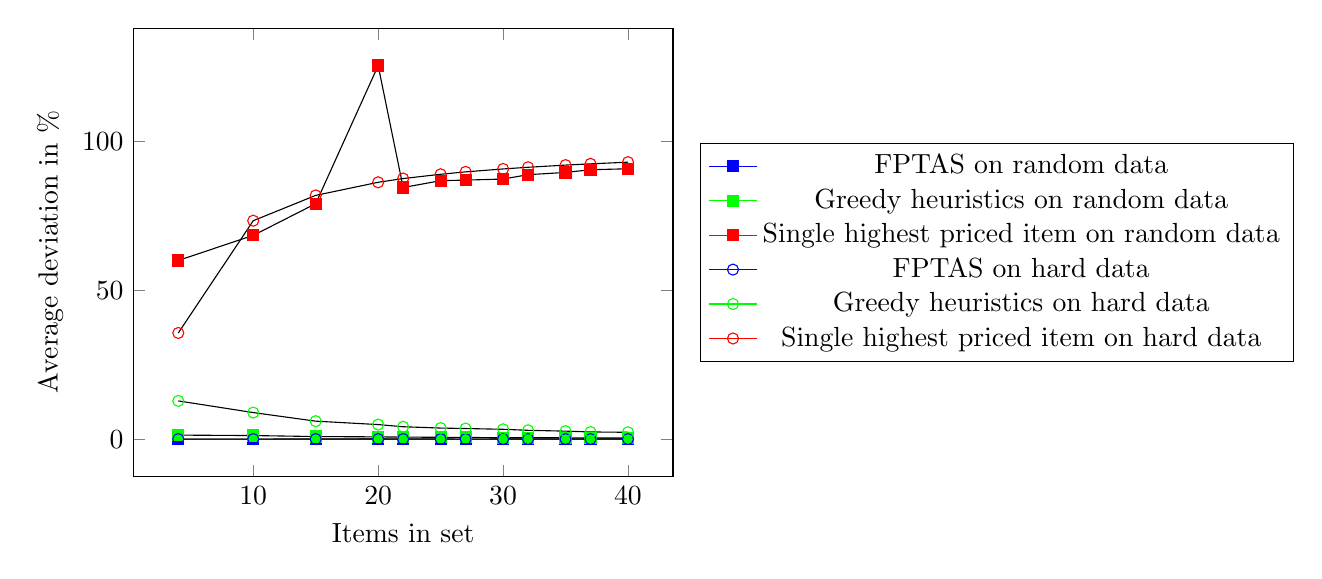
\begin{tikzpicture}
		\begin{axis}[
			xlabel=Items in set,
			ylabel=Average deviation in \%,
			scatter/classes={
				fptasN={mark=square*,blue},
				hungryN={mark=square*,green},
				singleN={mark=square*,red},
				fptasH={mark=o,blue},
				hungryH={mark=o,green},
				singleH={mark=o,red}
				}
			]
			\addplot[scatter,%
				scatter src=explicit symbolic]%
			table[meta=label] {
                x y label
                4 .095931 fptasN
                10 .085455 fptasN
                15 .091002 fptasN
                20 .145440 fptasN
                22 .089912 fptasN
                25 .091948 fptasN
                27 .091139 fptasN
                30 .089941 fptasN
                32 .092691 fptasN
                35 .092870 fptasN
                37 .093395 fptasN
                40 .094362 fptasN
			};
			\addplot[scatter,%
				scatter src=explicit symbolic]%
			table[meta=label] {
				x y label
				4 1.453410 hungryN
                10 1.304166 hungryN
                15 .968396 hungryN
                20 .860422 hungryN
                22 .778518 hungryN
                25 .724522 hungryN
                27 .691782 hungryN
                30 .529006 hungryN
                32 .596280 hungryN
                35 .557696 hungryN
                37 .469084 hungryN
                40 .481640 hungryN
			};
			\addplot[scatter,%
				scatter src=explicit symbolic]%
			table[meta=label] {
				x y label
				4 60.139400 singleN
                10 68.546800 singleN
                15 79.198600 singleN
                20 125.595400 singleN
                22 84.639200 singleN
                25 86.921000 singleN
                27 87.121200 singleN
                30 87.479400 singleN
                32 88.943600 singleN
                35 89.693800 singleN
                37 90.602800 singleN
                40 90.929800 singleN
			};
			\addplot[scatter,%
				scatter src=explicit symbolic]%
			table[meta=label] {
				x y label
				4 .123029 fptasH
                10 .127224 fptasH
                15 .130156 fptasH
                20 .129032 fptasH
                22 .129395 fptasH
                25 .128979 fptasH
                27 .127454 fptasH
                30 .128554 fptasH
                32 .129028 fptasH
                35 .129171 fptasH
                37 .128856 fptasH
                40 .128841 fptasH
			};
			\addplot[scatter,%
				scatter src=explicit symbolic]%
			table[meta=label] {
				x y label
				4 12.939740 hungryH
                10 9.023060 hungryH
                15 6.139760 hungryH
                20 4.991380 hungryH
                22 4.266580 hungryH
                25 3.821660 hungryH
                27 3.664740 hungryH
                30 3.409840 hungryH
                32 3.063500 hungryH
                35 2.788140 hungryH
                37 2.510400 hungryH
                40 2.398320 hungryH
			};
			\addplot[scatter,%
				scatter src=explicit symbolic]%
			table[meta=label] {
				x y label
				4 35.772200 singleH
                10 73.480400 singleH
                15 81.983600 singleH
                20 86.386000 singleH
                22 87.645200 singleH
                25 89.082000 singleH
                27 89.892600 singleH
                30 90.870400 singleH
                32 91.434800 singleH
                35 92.163000 singleH
                37 92.582000 singleH
                40 93.148600 singleH
			};
			\addlegendentry{FPTAS on random data}
			\addlegendentry{Greedy heuristics on random data}
			\addlegendentry{Single highest priced item on random data}
			\addlegendentry{FPTAS on hard data}
			\addlegendentry{Greedy heuristics on hard data}
			\addlegendentry{Single highest priced item on hard data}
		\end{axis}
	\end{tikzpicture}
\caption{Average deviation in approximation algorithms}
\label{plot:deviation}
\end{figure}
